\documentclass[logo,reportComp]{thesis}
\usepackage[python,pseudo]{mypackage}

\title{自然语言处理}
\subtitle{期中大项目:文本预测}
\school{数据科学与计算机学院}
\author{陈鸿峥}
\classname{17大数据与人工智能}
\stunum{17341015}
\headercontext{自然语言处理作业}

\let\emph\relax % there's no \RedeclareTextFontCommand
\DeclareTextFontCommand{\emph}{\kaiti\em}

\begin{document}

\maketitle
\tableofcontents

\newpage
\section{新闻内容抓取}
% 从国内主流新闻网站(如腾讯、新浪、网易等)的科技频道抓取新闻内容。
% 要求新闻语言为中文,发布日期为2019年1月1日以后。
% 数量至少为1000条。

新闻内容的抓取又可以分成以下的三个阶段:生成包含科技新闻页面的url列表,从url列表中下载对应的新闻文本,对原始新闻文本进行一些简单的处理。

源代码可见\verb'spider.py'。
下面将分别对这三个阶段进行说明。


\subsection{提取新闻链接地址}
新闻链接主要从网易科技的以下三个主页面进行抓取:
\begin{itemize}
    \item IT业界\_网易科技频道:\url{http://tech.163.com/special/it_2016/}\\
    第$X$个页面的地址为\verb'/it_2016_X',$X\in[1,20]$,每个页面有20条新闻。
    \begin{figure}[H]
        \centering
        
\includegraphics[width=0.7\linewidth]{fig/it_netease.png}
        \caption{IT业界\_网易科技频道}
    \end{figure}
    \item 滚动\_网易科技频道:\url{http://tech.163.com/special/gd2016/}\\
    第$X$个页面的地址为\verb'/gd2016_X',$X\in[1,20]$,每个页面有20条新闻。
    \begin{figure}[H]
        \centering
        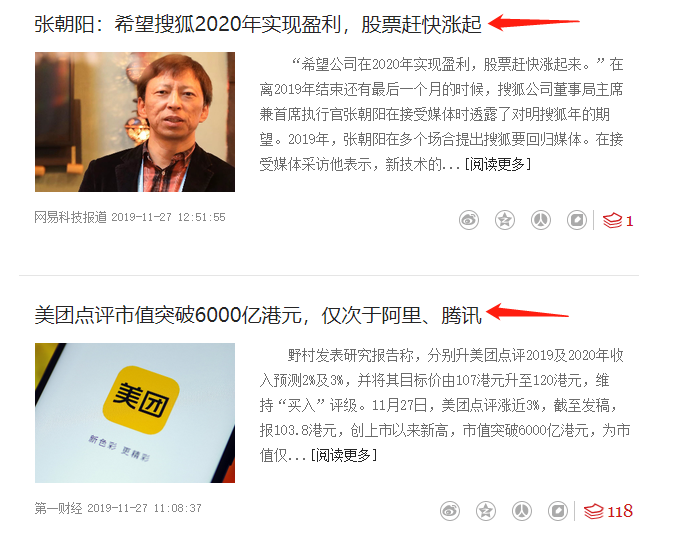
\includegraphics[width=0.7\linewidth]{fig/gd_netease.png}
        \caption{滚动\_网易科技频道}
    \end{figure}
    \item 原创报道\_网易科技:\url{http://tech.163.com/special/0009rt/ycbd.html}\\
    第$X$个页面的地址为\verb'/ycbd_i.html',$X\in[1,10]$,每个页面有100条新闻。
    \begin{figure}[H]
        \centering
        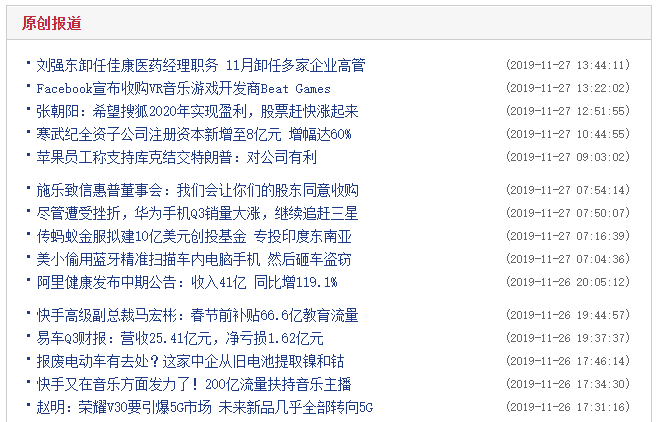
\includegraphics[width=0.8\linewidth]{fig/ycbd_netease.png}
        \caption{原创报道\_网易科技}
    \end{figure}
\end{itemize}
这三个页面的HTML结构比较清晰,且不需要不包含javascript代码通过后台数据库进行数据的动态生成,因此大大降低了爬虫抓取数据的难度。

在每一个入口页面找到内层文本标签中的\verb'href'标记,并将其中的链接提取出来,加上新闻标题一起写入\verb'csv'文件,即\verb'url.txt',如下图所示。
\begin{figure}[H]
\centering
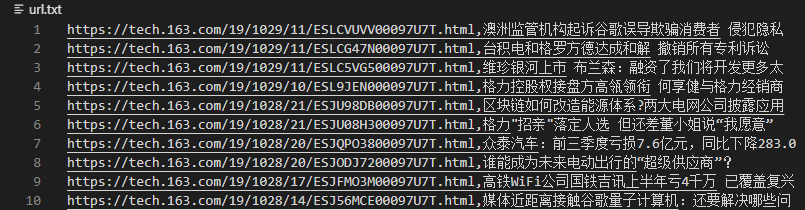
\includegraphics[width=\linewidth]{fig/url.png}
\caption{url.txt文件实例}
\end{figure}

\subsection{下载新闻文本}
我在程序中封装了以下函数
\begin{lstlisting}
def crawl(url,outfile_name)
\end{lstlisting}
其中\verb'url'为从上一阶段获得的每一条新闻的url地址,\verb'outfile_name'为输出文本的名字。

网易所有的新闻文本都会被封装在\verb'<post_text>'属性中,因此只需下载对应页面后,对HTML网页进行解析获取对应标签内容即可。

但要注意大多数网页可以用\verb'lxml'进行解析,但对于少部分网页,需要使用\verb'html.parser'配合\verb'gb18030'编码来处理中文。

\subsection{新闻数据处理}
对下载下来的原始新闻文本做一些简单的处理,包括:
\begin{itemize}
\item 删除行中的多余空格(用\verb'lstrip'和\verb'rstrip')
\item 删除网易新闻的标记,如``\_网易科技''、``网易科技讯''等
\item 删除其他无关字符,如\verb'@@LinkCard'
\end{itemize}

\subsection{实施细节}
这一部分主要采用Python的\verb'bs4'和\verb'request'包进行新闻内容的抓取,其他一些实现细节如下:
\begin{itemize}
\item 为避免网页的反爬虫机制,需要对爬虫进行伪装,因此需要自行设置网页请求头\verb'send_headers'
\item 在网页抓取时设置\verb'time_out',防止抓取网页时因为网速过慢等原因卡死整个程序
\item 读写文件时注意强制声明编码为\verb'utf-8'
\item 为了避免网页的重复抓取,采用\verb'os.path.isfile'判断文件是否存在,若某一新闻文件已经存在,则不再访问对应网页。
\item 使用Python的多进程库\verb'multiprocessing'\footnote{之所以不使用多线程,是因为Python的多线程机制非常鸡肋,同时没有线程池可以管理。而多进程相对比较成熟,且有进程池Pool统一进行管理。}并发抓取网页,加快任务执行速度。
\end{itemize}


\section{新闻数据预处理}
% 对新闻数据进行预处理(分句、分词、去噪)。
% 在这个过程中同时要完成建立词表的工作。
% 可以使用已有的一些中文分词工具。

新闻数据预处理在前一节已经完成了一部分,因此这里着重于中文的分词。
采用结巴分词(\verb'cut')工具,完整代码可见\verb'cut.py'。

核心代码如下所示。
\begin{lstlisting}
text = jieba.lcut(intext,cut_all=False)
\end{lstlisting}
这里采用了精确模式(\verb'cut_all=False'),可以确保一些词汇不会被分割得太细,如避免``人工智能''分割为``人工$\mid$智能'';同时采用\verb'lcut'可以使结果直接返回一个列表,而不是Python的迭代器。

除了前述的预处理工作,在本部分还进行了以下工作:
\begin{itemize}
\item 将多个空行换为单一空行,即
\begin{lstlisting}
intext = intext.replace('\n\n','\n')
\end{lstlisting}
\item 尽可能将不同的句子分置在不同的行中,即将在句号末换行。
\item 用\verb'collections.Counter'对分词后的列表进行计数,生成\verb'dict.txt'(这一部分在后面被移到各自的训练模型文件中)
\end{itemize}

生成预处理后的分词文件实例如下。
\begin{figure}[H]
\centering
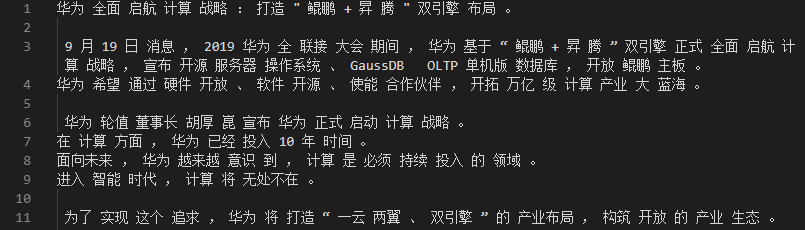
\includegraphics[width=\linewidth]{fig/jieba.png}
\caption{预处理后分词文件实例}
\end{figure}


\section{模型训练}
% 使用预处理后的新闻数据训练两个语言模型。
% 其一为简单的n-gram语言模型(n取2或者3)。
% 其二为基于RNN/LSTM/GRU的语言模型。
% 词典大小、网络和训练的超参数等可以自己指定。

在本次实验中,我使用预处理后的新闻数据训练了两个语言模型,一个为3-gram,另一个为LSTM,详细说明如下。

\subsection{n-gram模型}
n-gram模型为统计语言模型,我将其分成以下三个阶段进行模型生成及预测。
完整代码可见\verb'ngram.py'。

\subsubsection{去除停止词及加句子标记}
n-gram模型能够正常工作很重要一点在于去除停止词,这里我采用了\cite{bib:stopword}中的中文常用停止词列表。
通过判断某一单词是否在停用词列表中,然后决定是否将其保留。

同时,每读入一个句子需要在句子前面加上起始标记\verb'<BOS>',在句末加上终止标记\verb'<EOS>'。

\subsubsection{生成n-gram列表}
将上述去除停用词及加句子标记的文本重新读入后,调用\verb'generate_ngram'函数生成n-gram列表。
这里我采用了一种非常快速且巧妙的方法,通过对单词列表移位然后重新组合,即可得到对应的$n$元组。
再将这些$n$元组用空格连接,即可得到对应的n-gram。
\begin{lstlisting}
def generate_ngram(text,n):
    token = text.split()
    ngrams = zip(*[token[i:] for i in range(n)])
    return [" ".join(ngram) for ngram in ngrams]
\end{lstlisting}

在实际实施中,会在这个阶段生成三个n-gram列表,如下所示。
同时用用\verb'Counter'对列表内容进行计数。
将生成的计数结果用\verb'pickle'序列化处理,保存为\verb'pkl'方便后续直接读入使用。
\begin{itemize}
    \item 1-gram:实际上就是词表,在选词填空时将会从中进行选择
    \item n-gram:核心的n-gram模块,保存着所有的n-gram文本
    \item (n-1)-gram:用于实际计算中历史字串的索引
\end{itemize}

\subsubsection{模型预测}
对于每一个需要预测的句子,读入后先确定\verb'[MASK]'标记的地方,然后分为前后两个部分进行分词。
由于在模型生成中将停用词去除并添加了句首句末标记,因此在实际预测中也需要对预测的文本进行同样的处理。

通过遍历词表,每次选择一个词填入\verb'[MASK]'标记中,然后利用加性平滑(additive smoothing)通过下式计算最大似然概率
\[p(w_i\mid w_{i-n+1}^{i-1})=f(w_i\mid w_{i-n+1}^{i-1})=\frac{c(w_{i-n+1}^i)}{\sum_{w_i}c(w_{i-n+1}^i)}\]
其中,$\sum_{w_i}c(w_{i-n+1})$为历史串$w_{i-n+1}^{i-1}$在给定语料中出现的次数,即$c(w_{i-n+1}^{i-1})$,这也是为什么前面需要提前计算出(n-1)-gram。
从所有计算出的概率值中选择最大的那一个,其对应的词语即n-gram模型预测应该填入的词,核心代码如下。
\begin{lstlisting}
# calculate the maximum probability
rank = []
for mask in word_counter.keys():
    if mask in ["<BOS>","<EOS>"]:
        continue
    # only focus on the n-1 words before and after [MASK]
    new_text = seg_pre[-N+1:] + [mask] + seg_post[:N-1]
    text_gram = generate_ngram(new_text,N)
    gram_val = cal_ngram(text_gram)
    rank.append((gram_val,mask))
\end{lstlisting}

另外,注意到其实句子的其他部分对最终计算出来的概率值没有影响,真正对概率值有贡献的只有\verb'[MASK]'前后$n-1$的词的范围。
因此只考虑这$2n-1$个词将大大缩减预测时间。

具体实验结果可见第\ref{sub:n-gram}节。

\subsection{LSTM模型}
LSTM模型为神经网络模型,包括数据生成、模型搭建、训练和预测。
采用Pytorch v1.1进行模型搭建,并使用1块Titan V GPU进行训练。
由于一开始在Jupyter Notebook中进行代码编写及运行,因此建议直接访问\verb'lstm.ipynb'查看交互式数据。
另外,也可直接查看jupyter生成的代码文件\verb'lstm.py'。

\subsubsection{数据生成}
这里我编写了自己的\verb'TextDataset',其继承了\verb'torch.utils.data.Dataset'。
完整的类声明如下。
\begin{lstlisting}
class TextDataset(data.Dataset):
    """
    My own text dataset
    """
    def __init__(self, file_path, batch_size, seq_size):
        """
        Generate word indices and dictionary used for training

        file_path: The path of the folder storing all the news
        batch_size: size of one batch (used for batch training)
        seq_size: size of the sequence
        """
        text = []
        for i,file_name in enumerate(os.listdir(file_path),1):
            with open("{}/{}".format(file_path,file_name),"r",encoding="utf-8") as infile:
                for j,line in enumerate(infile):
                    text += line.split()
        word_counts = Counter(text) # {word: count}
        # sort based on counts, but only remain the word strings
        sorted_vocab = sorted(word_counts, key=word_counts.get, reverse=True)

        # make embedding based on the occurance frequency of the words
        self.int_to_word = {k: w for k, w in enumerate(sorted_vocab)}
        self.word_to_int = {w: k for k, w in self.int_to_word.items()}
        self.n_word = len(self.int_to_word)
        print('Vocabulary size', self.n_word)

        # turn all the words in the text to int
        int_text = [self.word_to_int[w] for w in text]
        num_batches = int(len(int_text) / (seq_size * batch_size))
        in_text = int_text[:num_batches * batch_size * seq_size]

        # shift right for one position to generate the 'label' Y
        out_text = np.zeros_like(in_text)
        out_text[:-1] = in_text[1:]
        out_text[-1] = in_text[0]

        # reshape X and Y (# of seq,seq_size)
        self.in_text = np.reshape(in_text,(-1,seq_size))
        self.out_text = np.reshape(out_text,(-1,seq_size))
        self.seq_size = seq_size

    def __len__(self):
        """
        Return the total number of samples
        """
        return len(self.in_text)

    def __getitem__(self, idx):
        """
        Generate one sample of the data
        """
        x = self.in_text[idx]
        y = self.out_text[idx]
        return x, y
\end{lstlisting}

\verb'TextDataset'中主要有三个函数:
\begin{itemize}
    \item \verb'__init__':将预处理过的所有新闻文本文件读入(注意这里采用了和ngram预处理同样的方法,\textbf{删除了标点符号和停止词,并添加句首句末标记}),然后构建词表,并对词频排序与单词之间建立一个一一映射,此时相当于把每一个单词都映射到一个整数序号值。
    将输入文本(X)右移一位即得到输出文本(Y),同时用\verb'reshape'对输入输出向量的维度进行改变,最后一维为序列长\verb'seq_size'。
    \item \verb'__len__':返回序列数目。
    \item \verb'__getitem__':根据\verb'idx'获得对应的序列。
\end{itemize}

封装好\verb'TextDataset'后,结合\verb'DataLoader'即可实现批训练数据的生成。
\begin{lstlisting}
train_set = TextDataset(flags.train_file_path, flags.batch_size, flags.seq_size)
train_loader = data.DataLoader(dataset=train_set,batch_size=flags.batch_size,shuffle=False)
\end{lstlisting}

\subsubsection{模型搭建}
在pytorch中搭建神经网络模型非常容易,只需定义好相关变量,并写好前向传播过程即可\footnote{后向传播由计算流图自动求导生成},代码模块如下。
\begin{lstlisting}
class RNNModule(nn.Module):
    """
    A basic LSTM model for text generation
    """
    def __init__(self, n_word, seq_size, embedding_size, lstm_size):
        super(RNNModule, self).__init__()
        self.seq_size = seq_size
        self.lstm_size = lstm_size

        # embed = nn.Embedding(vocab_size, vector_size)
        #   vocab_size is the number of words in your train, val and test set
        #   vector_size is the dimension of the word vectors you are using
        # you can view it as a linear transformation
        # the tensor is initialized randomly
        self.embedding = nn.Embedding(n_word, embedding_size)

        self.lstm = nn.LSTM(embedding_size, lstm_size, batch_first=True)
        self.linear = nn.Linear(lstm_size, n_word)

    def forward(self, x, prev_state):
        """
        Forward propagation
        """
        embedding = self.embedding(x)
        # used for next layer
        output, state = self.lstm(embedding, prev_state)
        # used for output
        logits = self.linear(output)
        return logits, state

    def zero_state(self, batch_size):
        """
        Used to make the state all zeros
        """
        return (torch.zeros(1, batch_size, self.lstm_size),
                torch.zeros(1, batch_size, self.lstm_size))
\end{lstlisting}

这里将输入向量做了词嵌入,映射到维度为\verb'vector_size'空间中的一个向量,然后用LSTM模型进行训练。

LSTM的模型如图\ref{fig:lstm-unit}所示\footnote{图源自Application of Long Short-Term Memory (LSTM) Neural Network for Flood Forecasting, \url{https://www.mdpi.com/2073-4441/11/7/1387}}。
\begin{figure}[H]
\centering
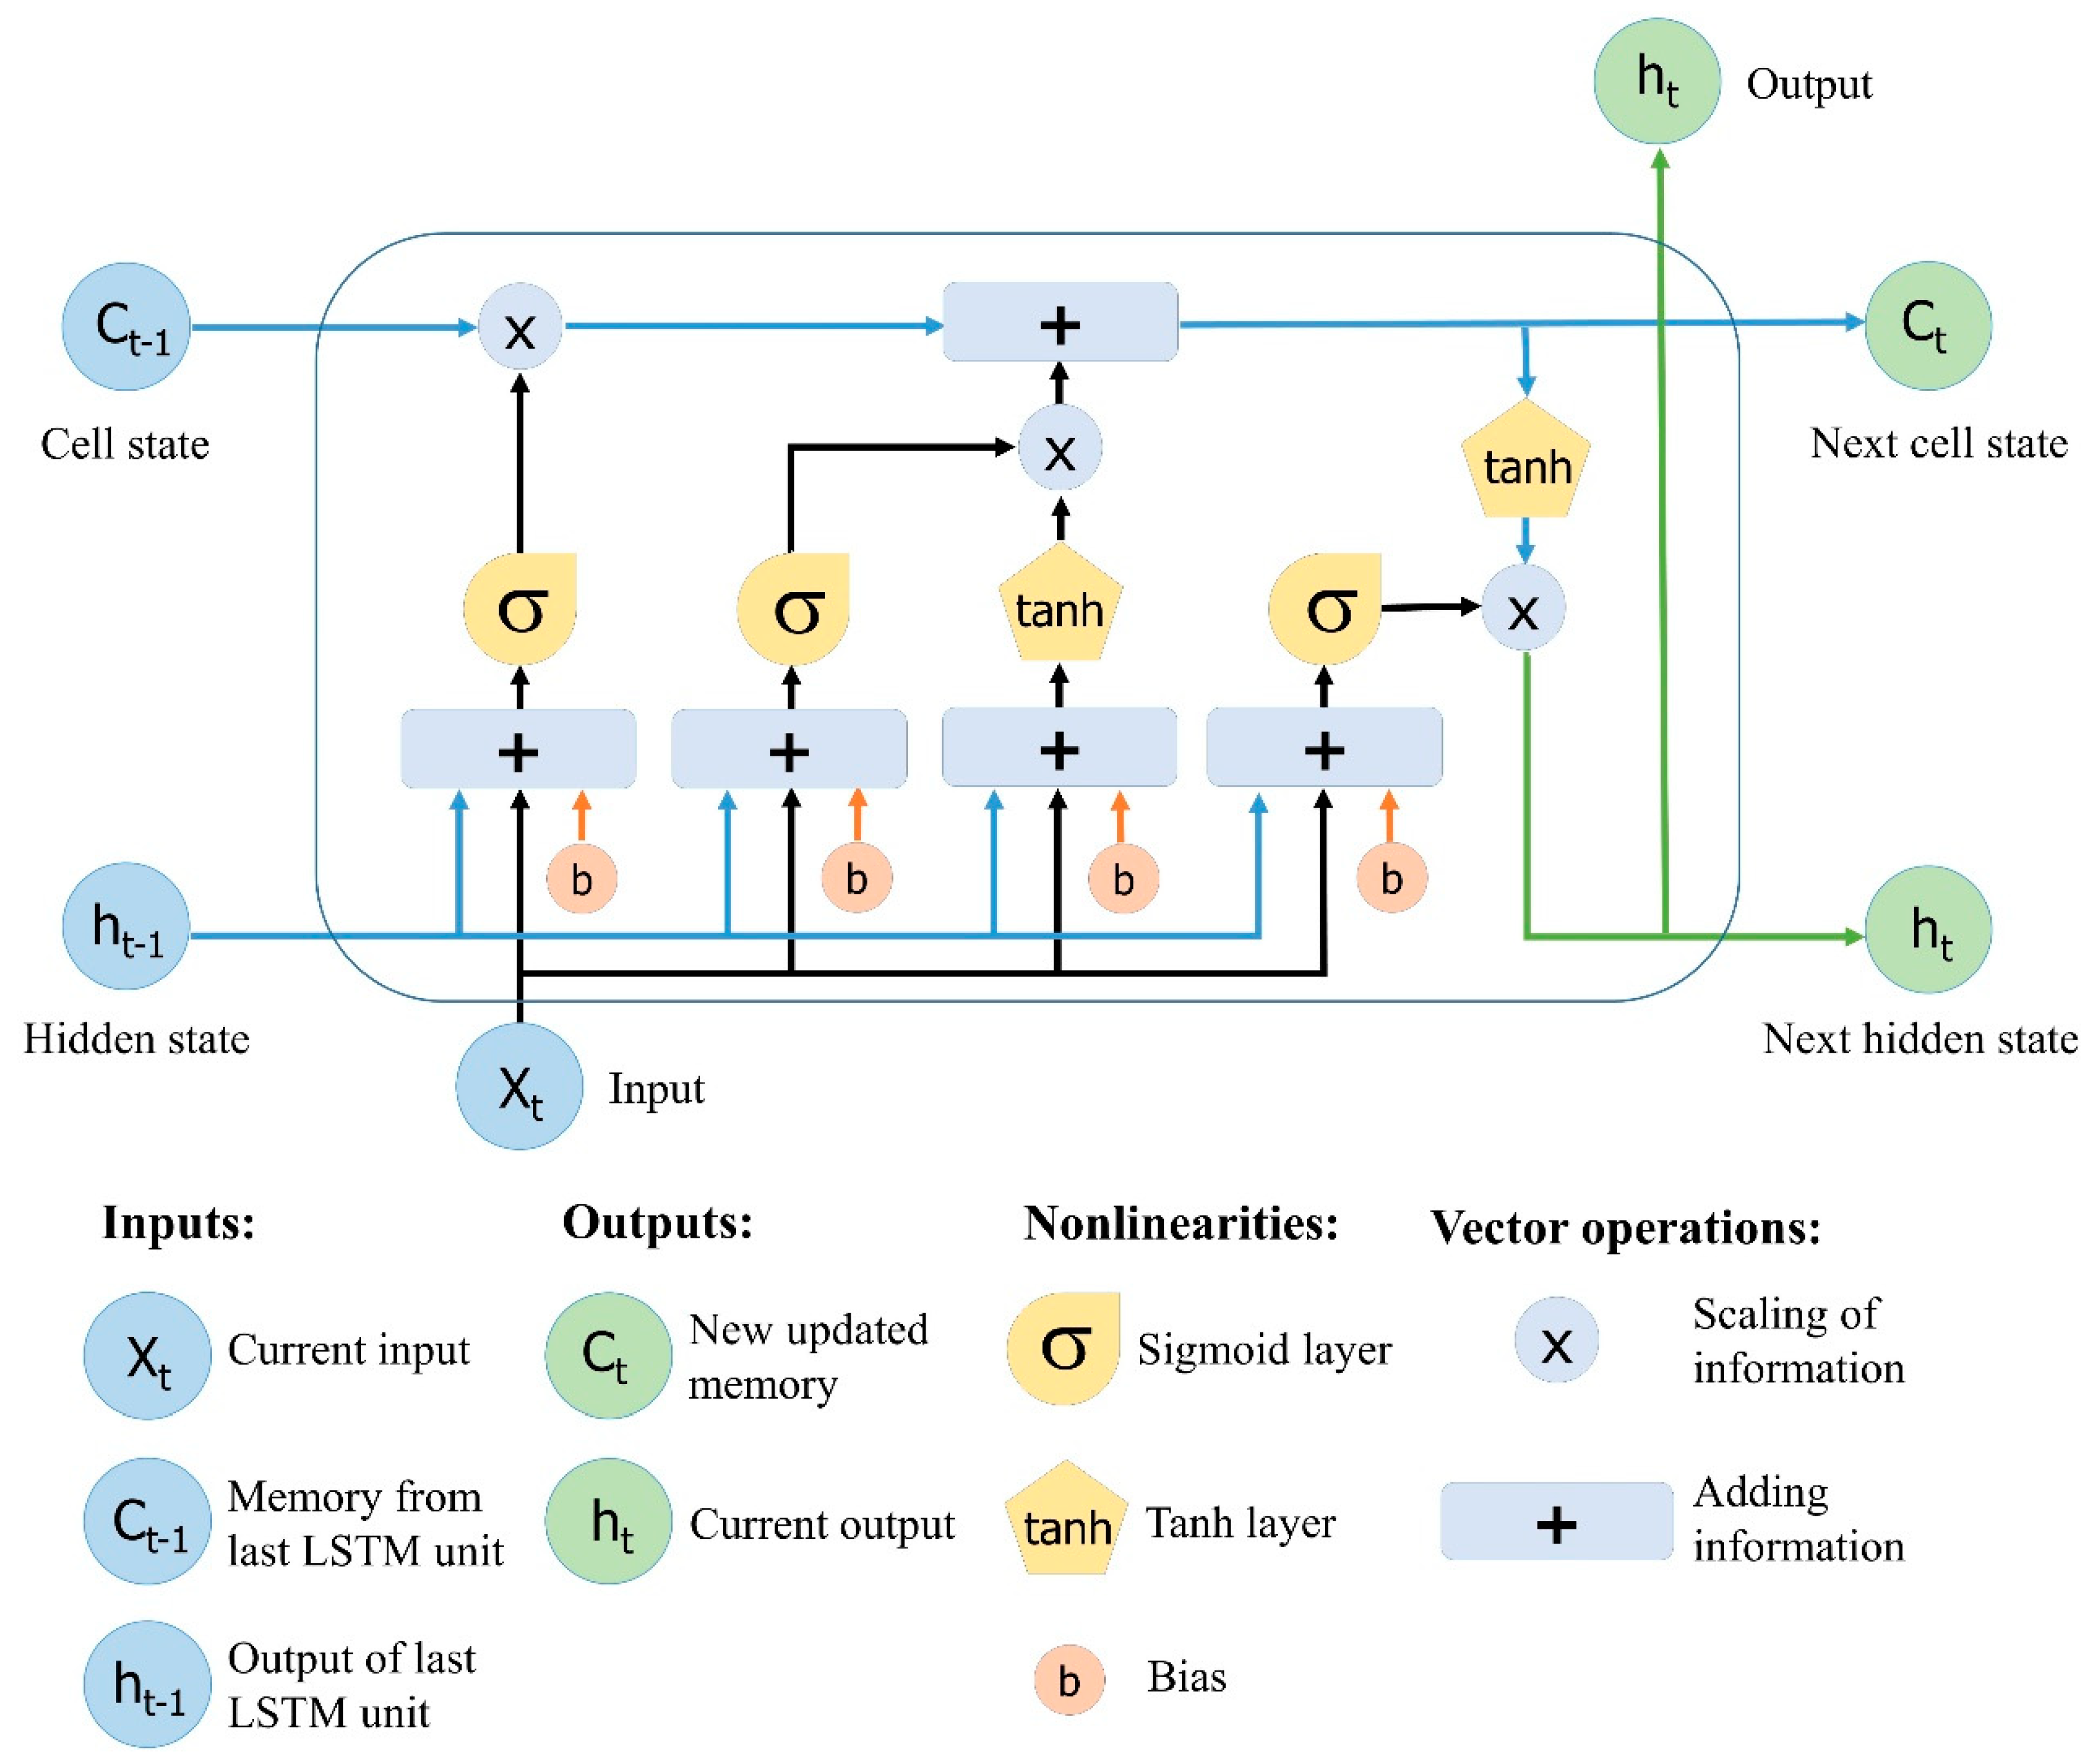
\includegraphics[width=0.8\linewidth]{fig/lstm-unit.png}
\caption{LSTM单元}
\label{fig:lstm-unit}
\end{figure}

因此前向传播主要包括横向纵向的传播,横向传播状态,纵向生成输出,即对应着下面这条语句。
\begin{lstlisting}
output, state = self.lstm(embedding, prev_state)
\end{lstlisting}

为提升模型的泛化能力,输出会再通过一个线性层,得到最终的输出向量。

\subsubsection{模型训练}
模型训练的核心代码如下所示,在每一轮训练中都会将所有数据进行批训练。
\begin{lstlisting}
for e in range(flags.num_epochs):
    state_h, state_c = net.zero_state(flags.batch_size)
    state_h = state_h.to(device)
    state_c = state_c.to(device)

    for step, (x, y) in enumerate(train_loader):
        iteration += 1
        net.train()

        optimizer.zero_grad()

        x = torch.tensor(x).to(device)
        y = torch.tensor(y).to(device)

        logits, (state_h, state_c) = net(x, (state_h, state_c))
        loss = criterion(logits.transpose(1, 2), y)

        # avoid delivering loss from h_t and c_t
        # thus need to remove them from the computation graph
        state_h = state_h.detach()
        state_c = state_c.detach()

        loss_value = loss.item()

        loss.backward()

        # avoid gradient explosion
        _ = torch.nn.utils.clip_grad_norm_(net.parameters(), flags.gradients_norm)

        optimizer.step()
        losses.append(loss_value)
\end{lstlisting}

这里采用了交叉熵作为模型好坏的评价指标,并使用Adam优化器对目标进行优化。
从代码中可以看出在每一次批迭代中主要过程如下:
\begin{enumerate}
\item 将优化器的梯度置零,在当轮训练中才进行梯度累加
\item 从\verb'DataLoader'中读取批数据,转换为\verb'tensor',并放置到CPU/GPU上
\item 利用LSTM进行前向传播,并计算损失(loss)
\item 将$h_t$和$c_t$从计算流图中分离,再进行梯度回传
\item 为避免梯度爆炸,采用梯度裁剪(gradient clip)\cite{bib:gradient_clipping}的方式对每轮迭代后的梯度进行重新缩放处理
\item 优化器在梯度方向上前进一步,进入下一轮迭代
\end{enumerate}
以上几个步骤不断迭代,直到模型收敛或达到最大训练轮数。

\subsubsection{模型预测}
预测的方式与ngram模型类似,只是将核心部分改为神经网络的推断,核心代码如下。
\begin{lstlisting}
def predict(device, net, question_str, n_word, word_to_int, int_to_word, top_k=5):
    """
    Use net to do the prediction
    Each time only one question_str is input
    """
    net.eval() # set in evaluation mode
    # find out the blank
    q_index = question_str.index("[MASK]")
    question_pre, question_post = question_str[:q_index], question_str[q_index+len("[MASK]"):]

    # cut the sentence
    seg_pre = generate_seg_lst(question_pre)
    seg_post = generate_seg_lst(question_post)
    seg_pre.insert(0,"<BOS>")
    seg_post.insert(len(seg_post),"<EOS>")

    # LSTM inference
    state_h, state_c = net.zero_state(1)
    state_h = state_h.to(device)
    state_c = state_c.to(device)
    for w in seg_pre:
        index = word_to_int.get(w,word_to_int["<BOS>"])
        ix = torch.tensor([[index]]).to(device)
        output, (state_h, state_c) = net(ix, (state_h, state_c))

    # get the topk prediction
    _, top_ix = torch.topk(output[0], k=top_k)
    choices = top_ix.tolist()

    # return the corresponding words
    return [int_to_word[x] for x in choices[0]]
\end{lstlisting}

步骤如下:
\begin{enumerate}
\item 对句子进行分割和分词,删除停止词、标点符号,添加句首句末标记
\item 将输入文本(\verb'[MASK]'前面的部分)转换为对应的词向量,输入LSTM进行前向推理,每一次都更新状态$h_t$和$c_t$
\item 预测输出\verb'[MASK]'处的词向量,选取最高的$k$个的值作为预测
\item 将词向量映射回对应的单词输出
\end{enumerate}

\subsubsection{其他实施细节}
\begin{itemize}
    \item 采用\verb'argparse'进行命令行参数的读入与操作(主要是一些模型的超参数及文件路径)
    \item 采用\verb'logging'模块对训练过程进行日志记录,以便跟踪存在的问题
    \item 采用\verb'time'模块对模型训练时间进行记录,同时可以预测剩余训练时间
    \item 采用\verb'torch.save(net.state_dict())'的方法保存模型参数,一方面可以防止训练过程中的模型丢失,另一方面又可以避免将整个模型存储下来的空间开销
\end{itemize}

\section{实验结果}
% 使用我们提供的测试集检验训练好的模型的性能。
% 我们提供的测试数据是在同一来源的新闻中随机抽取的100个句子,其中每个句子有一个词被挖空,要求预测出这些词。
% 例如:因为刷脸支付也得去打开手机接收验证码,所以还不如直接扫[MASK]更直接更方便。(标准答案:二维码)
% 预测的结果好坏仅作为最终的分数的参考,重点在实验过程。

在具体实验中我将数据集进行了扩增,共采用2296条新闻进行模型生成、训练与预测。

\subsection{n-gram模型}
\label{sub:n-gram}
实验中我分别使用了$n=2,3,4$的几种模型进行预测,完整的预测正确率可见图\ref{fig:accuracy},完整结果可见\verb'myanswer-ngram.txt'。
执行样例如图\ref{fig:ngram-top1}和图\ref{fig:ngram-top5}所示。

\begin{figure}[H]
\centering
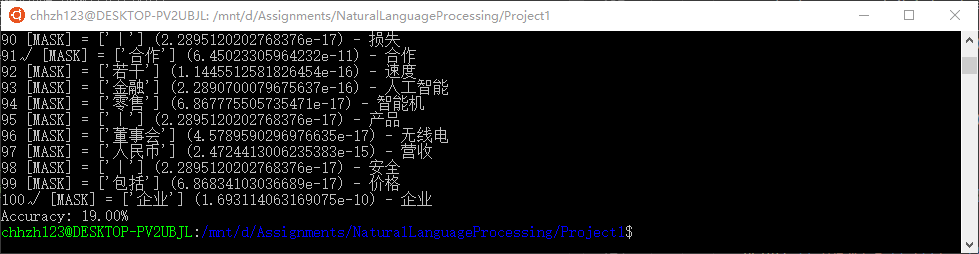
\includegraphics[width=\linewidth]{fig/result-ngram-top1.png}
\caption{3-gram模型(Top 1)执行过程与预测准确率}
\label{fig:ngram-top1}
\end{figure}
\begin{figure}[H]
\centering
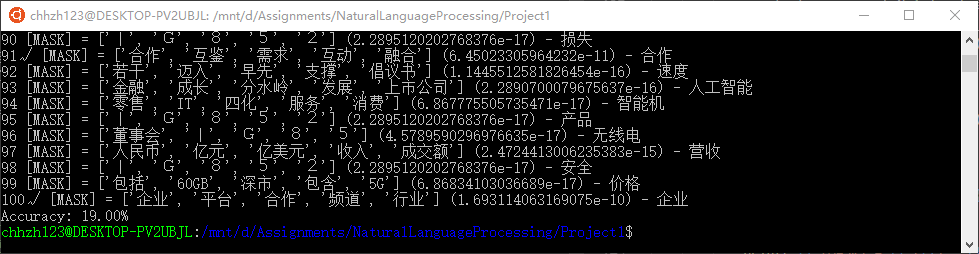
\includegraphics[width=\linewidth]{fig/result-ngram-top5.png}
\caption{3-gram模型(Top 5)执行过程与预测准确率}
\label{fig:ngram-top5}
\end{figure}

这里以3-gram的预测结果进行分析。
从上述图中可以看出3-gram的预测准确率是非常高的,达到了19\%,而且这19个全部在Top 1命中。

像预测值中出现的``$\mid$, G, 8, 5, 2''等是因为词表不够大,导致没有找到合适的词语填入,因此所有词语得到的预测概率都近似相同。
但可以预计,如果我们有足够大的词表,那么基于传统的统计模型进行文本预测依然可以做得很好。

接下来我们着重分析那些有正常的预测值的情况。
先看预测正确的情况,以第100条句子为例。
\begin{flushleft}
\kaiti 100 携程的目标是三年内成为亚洲最大的国际旅游企业,五年内成为全球最大的国际旅游企业,十年内成为最具价值和最受尊敬的在线旅游[MASK]。
\end{flushleft}
在这个空中,n-gram模型直接将在线旅游与\emph{企业/平台}联系在一起,并且给出了较高的预测值。
但其实这个空填\emph{平台}也没有太大问题,因为携程确实也可以被称为在线旅游\emph{平台},只是为了跟前文的\emph{国际旅游企业}照应,因此这里填\emph{企业}较优。

接下来再看看错误的情况,以第93、94条句子为例,这两个例子明显体现出统计模型的``缺陷''。
\begin{flushleft}
\kaiti 93 互联网和人工智能技术为全世界的各个国家都带来巨变。在这一方面,中国做得非常优秀,中国将互联网与[MASK]技术结合得“炉火纯青”,这些经验值得各个国家学习。
\end{flushleft}

第93句中由于大量语料都将\emph{互联网}和\emph{金融}相提并论,因此这里直接得出\emph{金融}为最高的预测值。
但是,n-gram的窗口明显没有将前一句中的\emph{人工智能}纳入考虑,故属于不能\textbf{具体情况具体分析},而只是生搬硬套以前的结论。

\begin{flushleft}
\kaiti 94 总之,5G将开启一个新智能机时代,而创新将是新智能机时代的第一发展动力,期待国产品牌在新[MASK]时代大有作为。
\end{flushleft}
同样,对于第94句来说,\emph{新零售时代}和\emph{IT时代}都是没有语病的,但是放在句子中却会产生不对应,因为前文提及的是\emph{新智能机时代},因此后面也应该填\emph{智能}时代。

\subsection{LSTM模型}
\label{sub:lstm}
LSTM模型中使用的超参数如表\ref{tab:lstm_hyperparam}所示,训练时间与超参数选择相关,由8分钟到18分钟不等。
\begin{table}[H]
\caption{LSTM模型超参数}
\label{tab:lstm_hyperparam}
\centering
\begin{tabular}{|c|c|c|}\hline
参数 & 变量名 & 数值\\\hline
序列长 & \verb'seq_size' & 32\\\hline
批大小 & \verb'batch_size' & 64\\\hline
词嵌入维度 & \verb'embedding_size' & 128\\\hline
LSTM隐态维度\cite{bib:pytorch_lstm} & \verb'lstm_size' & 128\\\hline
梯度裁剪阈值\cite{bib:gradient_clipping} & \verb'gradients_norm' & 5\\\hline
训练轮数 & \verb'num_epochs' & 40\\\hline
优化器学习率 & \verb'learning_rate' & 0.001\\\hline
\end{tabular}
\end{table}

训练过程中的损失函数变化如图\ref{fig:lstm-loss}所示,可以看到损失函数在不断下降,说明模型在不断变好。
\begin{figure}[H]
\centering
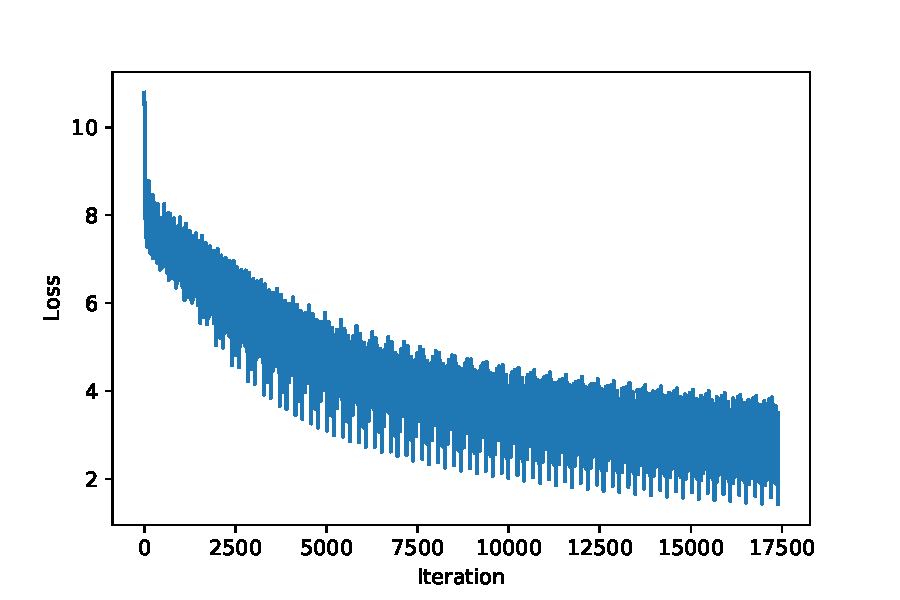
\includegraphics[width=0.8\linewidth]{fig/train_loss.pdf}
\caption{LSTM训练损失(loss)变化}
\label{fig:lstm-loss}
\end{figure}

对应的Top 1、Top 3、Top 5预测准确率如图\ref{fig:lstm-acc}所示,训练到后期模型已经开始有过拟合的趋势(Top 3和Top 5准确率下降)。
\begin{figure}[H]
\centering
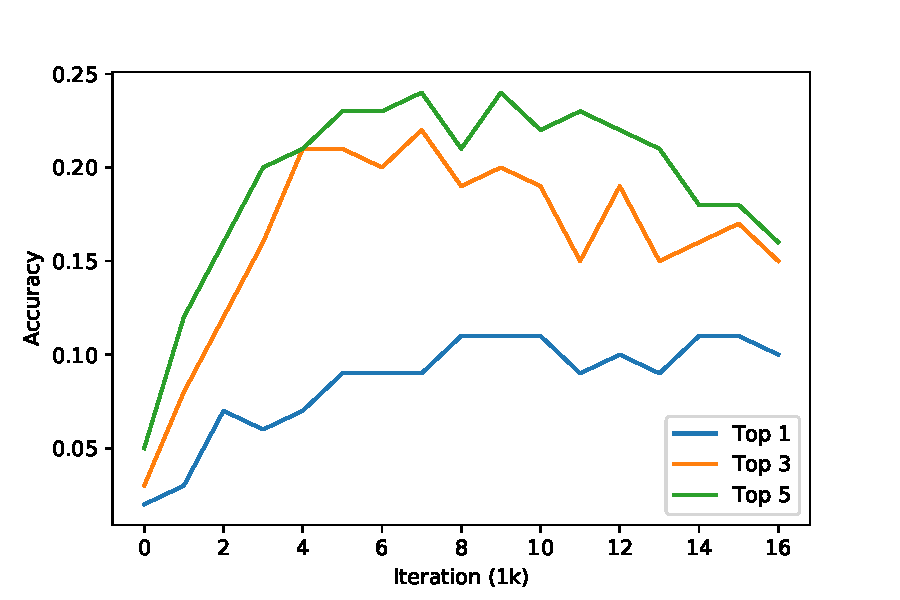
\includegraphics[width=0.8\linewidth]{fig/acc-iter.pdf}
\caption{LSTM训练预测准确率变化}
\label{fig:lstm-acc}
\end{figure}

实际推断样例如图\ref{fig:lstm-top1}和图\ref{fig:lstm-top5}所示(完整结果可见\verb'myanswer-lstm.txt'),可以看到LSTM模型的Top 1的准确率并不高,只有11\%;而Top 5的预测准确率才超过传统的统计模型。
另外,由于LSTM模型是预训练的,而n-gram模型是在线推断,因此相比起n-gram,LSTM的预测速度远超n-gram模型。
\begin{figure}[H]
\centering
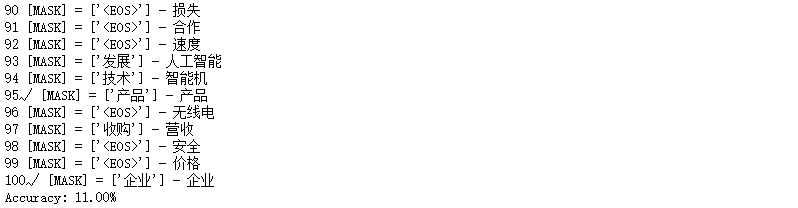
\includegraphics[width=\linewidth]{fig/result-lstm-top1.png}
\caption{LSTM模型(Top 1)执行过程与预测准确率}
\label{fig:lstm-top1}
\end{figure}
\begin{figure}[H]
\centering
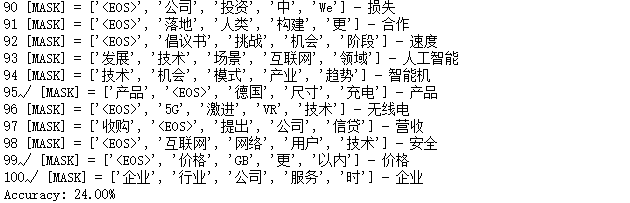
\includegraphics[width=\linewidth]{fig/result-lstm-top5.png}
\caption{LSTM模型(Top 5)执行过程与预测准确率}
\label{fig:lstm-top5}
\end{figure}

在实际操作中如果某个词语在词表中找不到,则我将其直接映射为\verb'<BOS>'对应的向量,因此这里出现的\verb'<BOS>'和\verb'<EOS>'同样是由于词表太小不够导致的预测错误,而非模型本身的问题。

接下来同样进行样例分析。
\begin{flushleft}
\kaiti 95 面对山河日下的情况,漫步者推出旗下定位于高端无线便携音响的[MASK],聚焦打造售价、利润率更高的高端产品线,以期提高利润率。
\end{flushleft}
第95条句子可以将\emph{音响}与\emph{产品}联系在一起,这是非常不容易的,在传统的统计模型中就很难做到这一点。
同时后面的预测值中还有\emph{充电}等字眼,这是与\emph{无线}进行了匹配。

\begin{flushleft}
\kaiti 98 腾讯安全平台部作为专注腾讯企业内部安全的团队,也把十余年腾讯自身安全最佳实践对外开放赋能,并逐步把[MASK]能力向腾讯云上开放,做好产业互联时代的数字化安全助手。
\end{flushleft}
第98条句子虽然整句话都在提及互联网相关的内容,但是神经网络显然将其定位得太宽泛,\emph{互联网}、\emph{网络}、\emph{用户}、\emph{技术}确实在相关语料中常常一起出现,但是具体到这一个句子中却不是正确的匹配项。
因为前面提及到\emph{安全},因此后文也应该用\emph{安全}相匹配。

从这些例子中也可以看出神经网络模型更具灵活性,即使对于同样的输入值,由于处在不同的状态(上下文),因此也会预测出不同的结果。

\subsection{综合比较}
所有模型的预测准确率如图\ref{fig:accuracy}所示。
\begin{figure}[H]
\centering
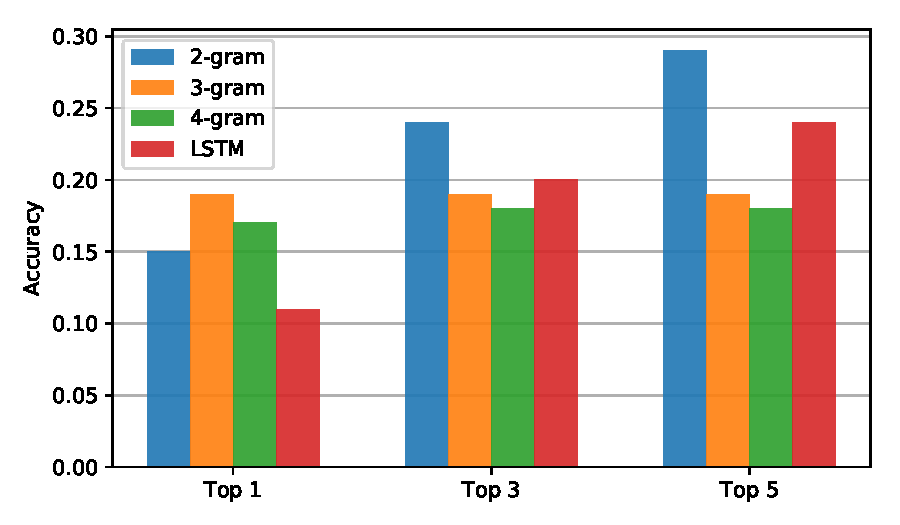
\includegraphics[width=0.8\linewidth]{fig/accuracy.pdf}
\caption{预测准确率比较}
\label{fig:accuracy}
\end{figure}

从图\ref{fig:accuracy}中,我们可以得到以下结论:
\begin{itemize}
\item 在Top 1情况下,3-gram的预测精度最高,达到19\%;Top 3情况下,2-gram的预测精度最高,达到24\%;Top 5情况下,2-gram预测精度最高,达到29\%。
\item 传统的统计模型并非一无是处,从这个实验结果来看似乎是反直觉的---2-gram模型的预测精度竟然始终高于神经网络模型,同样也比3-gram和4-gram模型要好很多。
虽然2-gram采用非常极端的贪心算法(断章取义),但是对于这种小样本预测效果反而是最好的。
\item n-gram模型采用更大的窗口$n$将使得模型更加稳定,基本上能够在Top 1预测出来的结果都是十分确定的,而其他没预测出来的通常就是词表中找不到的词语。
\item LSTM的Top 1、Top 3、Top 5的预测精度分别为11\%、20\%和24\%。
虽然在这个实验中并不是很惊艳,但是从预测结果来看,LSTM的泛化能力最强,推断时间更快,且更能依照不同句子的特性做出适应性的推断。
\item 随着Top k的$k$值不断增加,各个模型的预测准确率都在不断提升。这说明模型很多时候并没有办法做到精确匹配,但是如果放宽条件,其预测准确率还是可以接受的。
\end{itemize}

\section{总结与思考}
这次项目让我对整个数据收集、处理、分析、建模的全过程有了深入的了解,同时也对自然语言处理的原理和理论有了更进一步的理解。

从这次项目中得到最大的体会就是\textcolor{red}{\textbf{有多大的人工,就有多大的智能}}。
在软件2.0时代\cite{bib:software},我们输入给程序的不再是算法,更加关键的是训练数据;以前程序编译出来的是机器指令,而现在则变成了网络的学习参数。
以前算法决定了模型的性能,而现在则是\textbf{数据规模、模型复杂性}决定了其性能。
随着输入数据规模的不断增大,神经网络训练出来的效果也会变得更好。

从这次实验中也可以看出,无论是统计模型还是神经网络模型其实都是无关语法的,不需太多前置知识,更加容易搭建且达到很高的精度。
相比起n-gram,神经网络模型更加是小白都可以搭。
只要模型没有问题,什么数据丢进去训练就好了(甚至不需要做停止词消除或其他的一些预处理,尽管会有影响),神经网络总能拟合到一个不错的结果,关键在于\textbf{超参数的选择与调整}上。
这体现了神经网络强大的拟合能力,也体现了软件2.0时代与软件1.0时代的巨大区别。

关于这两个模型的问题在前文实验中已经提及,这里再进行总结:
\begin{itemize}
\item 准确率:这是衡量模型性能最重要的指标,由于训练样本太小,测试样本也太小,其实是很难看出什么的。
但有一个明显的趋势在于,当数据量加大时,对于两个模型来说都有着巨大的提升空间。
只要语料及词表足够大,这两种模型应该都能达到很好的预测效果。
\item 推理能力:无论是n-gram还是LSTM其实都是按照既定的统计方法进行预测,它并不具有真正的智慧,或者说不具有推理能力。
比如前文举的几个案例分析,都是句子中的前半句提及了某样事物,后半句就进行复现,对于人类来说这是很明显的事情,但对于机器来说却非常困难。
即便是LSTM已经将过往历史很好地进行记录,但是遇到这种问题还是有些捉襟见肘。
不过这有点偏阅读理解的范畴,可能有一些更好的语言模型进行处理,这可以是后续的研究方向。
\item 泛化能力:虽然2-gram在本次实验中取得很好的成绩,但这明显是一种鼠目寸光、断章取义的行为,只通过前后两个词而不是通过整个句子的意思来填空显然是不可取的。
虽然LSTM能够对整个句子进行分析,但一旦句子变得很长,它也很难分析清楚前后关系。
另外,对于这两个模型来说,一个很重要的问题都是没有办法很好解决不在词表中的词语,但显然我们也不可能建立一个足够大的词库涵盖所有的情况,因此需要有更好的方法来处理这种没出现过的情况。
泛化也和推理密切相关,想像``太阳从东边升起''这一句子,将中间一词``东''挖去,如果机器通过足够多的统计数据知道\emph{太阳}和\emph{东}必然一起出现,那之后的例子中这两者在一起的概率都会被设得很大。
但是如果在这一个句子后面加一些内容,如``太阳从[MASK]边升起是错的'',这时就不能填\emph{东}了,而需要通过后文的推理得出填写其他的词语。(不过这可能扯得有点远了,会涉及到知识表示与推理的内容)
\end{itemize}

总的来说,本次实验既让我熟悉了大数据分析的整个流程,又加深了对自然语言处理语言模型的理解。
虽然步骤非常繁杂,但整个过程还是非常有趣的。

\begin{thebibliography}{99}
\bibitem{bib:stopword} 中文常用停止词列表,\url{https://github.com/goto456/stopwords}
\bibitem{bib:colah} Colah, \url{https://colah.github.io/posts/2015-08-Understanding-LSTMs/}
\bibitem{bib:pytorch} Pytorch tutorial, \url{https://pytorch.org/tutorials/beginner/nlp/sequence_models_tutorial.html}
\bibitem{bib:pytorch_lstm} Pytorch nn.LSTM, \url{https://pytorch.org/docs/stable/nn.html\#torch.nn.LSTM}
\bibitem{bib:gradient_clipping} How to Avoid Exploding Gradients With Gradient Clipping, \url{https://machinelearningmastery.com/how-to-avoid-exploding-gradients-in-neural-networks-with-gradient-clipping/}
\bibitem{bib:text_generation} Text Generation With Pytorch, \url{https://machinetalk.org/2019/02/08/text-generation-with-pytorch/}
\bibitem{bib:lstm} Language Modelling and Text Generation using LSTMs - Deep Learning for NLP, \url{https://medium.com/@shivambansal36/language-modelling-text-generation-using-lstms-deep-learning-for-nlp-ed36b224b275}
\bibitem{bib:software} Kunle Olukotun, \emph{Designing Computer Systems for Software 2.0}, ISCA Keynote, 2018
\end{thebibliography}

\end{document}
% 5. 撰写详细的实验报告,内容至少有如下几点,最好图文并茂:
% 对新闻数据爬取的过程。
% 对爬取的数据进行预处理的过程。
% 建立模型和训练的过程、训练中的各种指标变化。
% 使用我们提供的数据进行预测的过程、预测的结果示例。
% 总结与思考(遇到的困难及采用的解决方法、后续改进方向等)。

% 届时服务器下将有三个文件夹,分别是“新闻数据”、“预处理数据”与“代码与报告”。在相应的DDL之前,把需要提交的所有文件打包成姓名_学号.zip上传到对应文件夹中。
% 此外还有一个“相关资料”文件夹存放我们提供的资料。测试数据以及提交作业示例在晚些时候会上传至其内供下载。

% 10月31日:提交爬取的新闻数据。
% 压缩包内应包含1000个文本文件,分别命名为1.txt到1000.txt,其中每个文件内容为纯文字的新闻原文。
% 如果采用了多于1000条新闻数据,也只需要提交1000条即可。(需在报告中指明使用了多少训练数据)

% 11月11日:提交对新闻数据预处理的结果。
% 压缩包内应包含1001个文本文件。
% 其中1000个文本文件分别命名为1.txt到1000.txt ,文件的每行是新闻原文中的一个句子分词后的结果(以空格分隔),要求与上一步提交的新闻内容相对应。
% 还有一个文本文件为你预处理后构建的词表,文件每行为用空格隔开的序号以及单词。

% 11月30日:提交全部试验代码与实验报告。
% 压缩包内应包含:
% 一个文件夹,其中包括所有你编写的代码。
% 一篇pdf格式的实验报告,内容如前所述。
% 一个名为prediction.txt的文本文档,其有100行,第i行的内容为第i个测试样本中你预测出的一个词(你也可以在一行中按可能性顺序展示多个你预测出来的词,用空格隔开)。

% 爬取数据:20分
% 预处理数据:20分
% 训练和测试语言模型:30分
% 撰写报告:30分

% 在n-gram模型中,去掉停止词能节省资源、提高效率。
% 可参考\url{https://github.com/goto456/stopwords}。

% 显卡资源不足时,可考虑采用梯度累积的方法进行训练。
% 没接触过深度学习的同学可以先做Pytorch官网的tutorials,有个初步了解。
% 可以考虑尝试用BeautifulSoup进行html内容分析。